\chapter{Implementace}

V předchozí kapitole jsme navrhli strukturu, které se náš projekt bude držet. Stejně tak již víme, jakým způsobem bude se systémem interagovat hráč. Nyní můžeme přistoupit k jeho implementaci.

V této kapitole zběžně představíme, jak jsme celkově při implementaci postupovali, zevrubněji pak vylíčíme, jak jsme přistupovali k řešení překážek, které nám postavil do cesty zejména fyzikální subsystém. 

Podrobnou programátorskou dokumentaci k jednotlivým komponentám psanou v anglickém jazyce lze nalézt v příloze. Zvolili jsme pro ni standardní formát dokumentačních komentářů exportovaných do souboru XML, protože ten podporuje pohodlnou integraci s IDE (např. použití v našeptávači).

\subsubsection*{Závislosti}
Naše řešení používá několik externích knihoven. S tvorbou kosmetických efektů vypomohla knihovna DOTween \cite{DoTween}. Dále Math.NET Numerics \cite{MathDotNetNumerics} poskytlo stabilní a dobře testovaný nástroj k řešení soustav lineárních rovnic. Repozitoř SubclassPropertyDrawer \cite{SubclassPropertyDrawer} umožnila pohodlnou editaci jednotlivých SwordMovement.Modules v editoru. 

Dále je třeba poděkovat uživatelům unity fóra \cite{InvertReverseUIMask}, které pomohlo s implementací grafické reprezentace healthbaru.

Největší díky však patří github uživateli \textit{mstevenson}, jehož práce \cite{ConfigurableJointExtensions} citelně pomohla s pochopením chování cílové rotace na jointech - bez kterého by implementace zásadní části této práce nebyla možná.


\section{Implementace základních komponent}

Objektový návrh základních entit našeho systému již známe z předchozí kapitoly. Zde si podrobně nastíníme implementaci \textbf{šermíře} a jeho \textbf{meče} - nejprve vnitřní implementaci šermíře, potom meče, následně kosmetickou stránku šermíře (ta operuje víceméně odděleně od jeho základního fungování) a nakonec toto vše protkáme damage systémem. 

Vynecháme algoritmy jednotlivých modulů ovládání - ty jsme již podrobně nastínili v \ref{interfacesSwordMovementModulesSubsection} - a rovněž pro objekt kořenu hierarchie je implementace natolik přímočará, že se jím zde nebudeme zaobírat. 


\begin{figure}[p]\centering
  \center
  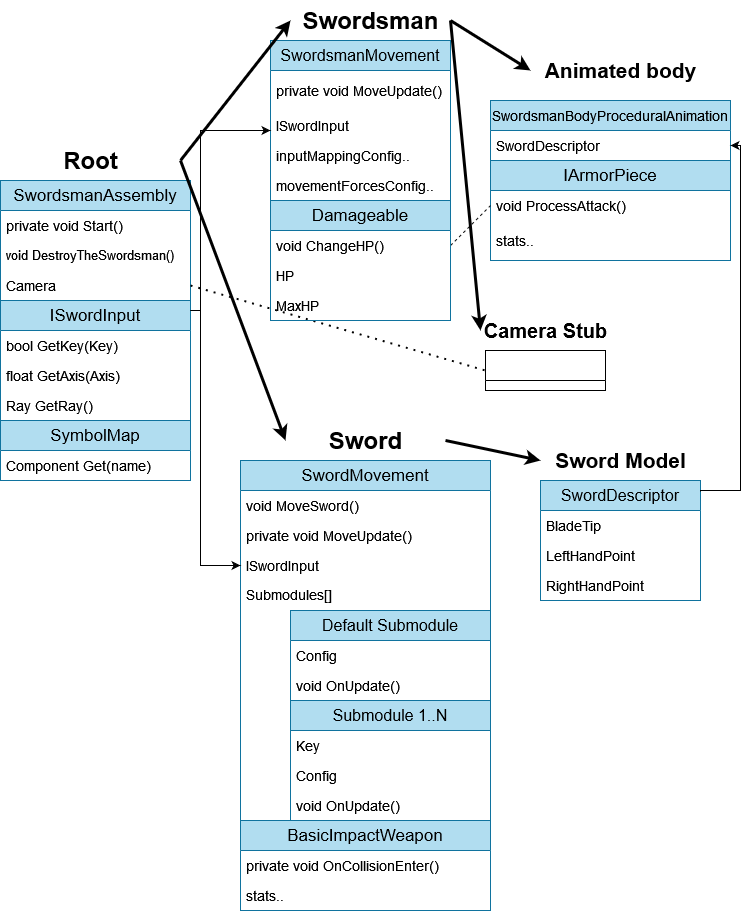
\includegraphics[width=145mm]{../img/Structure-diagram.png}
  \caption{Diagram znázorňující strukturu našeho systému - zopakování}
  \label{obr05:objectModelDiagramReprise}
\end{figure} 

\pagebreak

%------------------------------------------------------------------------------------------------------------------------------------------------------------------------------------------------------------------------------------------------------------%
 % xxxxxxxxxxxxxxxxxxxxxxxxxxxxxxxxxxxxxxxxxxxxxxxxxxxxxxxxxxxxxxxxxxxxxxxxxxxxxxxxxxxxxxxxxxxxxxxxxxxxxxxxxxxxxxxxxxxxxxxxxxxxxxxxxxxxxxxxxxxxxxxxxxxxxxxxxxxxxxxxxxxxxxxxxxxxxxxxxxxxxxxxxxxxxxxxxxxxxxxxxxxxxxxxxxxxxxxxxxxxxxxxxxxxxxxxxxxxxxxxxxxxxxxx %
%------------------------------------------------------------------------------------------------------------------------------------------------------------------------------------------------------------------------------------------------------------%


\subsection{Šermíř}

Šermíř je herní objekt, který reprezentuje hráče v herním světě. Potřebujeme od něj, aby byl schopen se pohybovat po herním světě a umožnil hráči skrze své oči nahlížet na svět. 

Instrukce od hráče bude přijímat z přidělené instance ISwordInput.

\subsubsection*{Pohyb}

Zásadním rozhodnutím, které jsme učinili, bylo implementovat šermíře jako \textbf{nekinematické Rigidbody}, ovládané čistě skrze fyzikální systém působením sil. 

\textit{Nejde o standardní postup - typicky je ve hrách pohyb postavy řešen přímo ze skriptu upravováním její polohy, postava může působit silami na okolní předměty, ale ne obráceně. Důvody jsou zřejmé - tvůrci hry takto získají větší kontrolu, která jim umožní ručně ladit pohyb postavy pro optimální hráčský zážitek; dále je často výslovně nevhodné, aby na hráčskou postavu působily silami okolní kolidující předměty - především při pohledu z 1. osoby, kdy hráč o převážně části svého těla nemá přehled - nezpozorovaná kolize, která postavu odmrští, pak může působit dojmem glitche. Unity pro tento standardní přístup poskytuje vyladěnou komponentu CharacterController.}

\textit{Pohyb hráče skrze fyzikální systém jsme zvolili zkrátka proto, že se zdál jako zajímavá oblast hodná prozkoumání. Přináší netriviální výzvy v oblasti zaručení stability hráčské postavy a responsivity ovládání. Na druhou stranu má šanci nám poskytnout další element navíc k meči, který může umocnit hráčovy možnosti fyzikální interakce s okolním prostředím\footnote{Např. s jeho přítomností můžeme zadarmo implementovat jednoduché fyzikální hádanky ala vyvažovací lávka v 2.misi Half-Life 2 \cite{HalfLife2}} a s nepřátelským mečem.}

Jak jsme tedy postupovali? Do herního objektu odpovídajícího hráči jsme umístili komponentu Rigidbody. Váhu jsme nastavil na 60 - cca odpovídající pro typického člověka, jinak jsme ponechali výchozí hodnoty. Pro účely kolizí s herním prostředím jsme vytvořili potomka obsahujícího jednoduchý CapsuleCollider se standardně používanými rozměry 2 x 0.5. Kapsle do sebe zhruba obsáhne šermířův model, ale nemá žádné ostré hrany, o které by se šermíř mohl zadrhávat při pohybu členitým terénem. Kolizní vrstvy jsme nastavili tak, aby tato kapsle kolidovala s terénem, ale ne s nepřáteli ani jejich zbraněmi.

Takto tedy vypadá fyzikální reprezentace šermíře, nyní k jejímu ovládání. Pro to jsme již určili zodpovědnou komponentu \textbf{SwordsmanMovement}. 

Konkrétní metody pohybu, které podporuje, jsou:
\begin{itemize}
  \item \textbf{Chůze dopředu/dozadu} - jednoduchý posun dopředu o kladnou nebo zápornou vzdálenost
  \item \textbf{Úkrok doleva/doprava} - jenoduchý posun doprava o kladnou nebo zápornou vzdálenost
  \item \textbf{Natočení se doleva/doprava} - rotace kolem šermířovy vertikální osy o kladný nebo záporný úhel, mění význam \textit{dopředu} a \textit{doprava}
  \item \textbf{Skákání} - okamžité aplikování impulzu na tělo hráče, pouze pokud hráč stojí na zemi
\end{itemize}

Pro každou z těchto akcí komponenta umožňuje nakonfigurovat vstupní osu, ze které budou funkcí ISwordInput.GetAxis() čteny instrukce (čísla v intervalu [-1;1]), dále rovněž číslo udávající rychlost pohybu. Pro skok je konfigurována aktivační klávesa a vektor síly impulzu.

\subsubsection*{Pohyb - Lineární pohyb}

Naivním přístupem k pohybu hráče by bylo zkrátka každý FixedUpdate přečíst hodnotu na příslušné ose, tu vynásobit s rychlostí, z této finální rychlosti získat sílu (nazvěme ji \textit{targetMovement}) vynásobením s vektorem udávajícím směr (dopředu/doprava), a tu aplikovat pomocí rigidbody.AddForce(targetMovement).
Tento přístup hráčem skutečně pohybuje ve správném směru, ne však způsobem, jaký bychom chtěli. Každá změna pohybu má pomalý rozjezd a jakmile se rozjede, dostat se z ní zpátky trvá stejně dlouho. Dlouhodobým pohybem v jednom směru šermíř stále zrychluje (hranicí je až rychlost světla). Rovněž se šermíř nijak nesnaží odolávat kolizím, které na něj působí. 

Řešením je vypočítanou hodnotu \textit{targetMovement} neinterpretovat jako sílu, ale jako cílovou rychlost šermíře. Aktuální rychlost šermíře lze získat jako \textit{rigidbody.velocity}. Spočítáme tedy \textit{targetMovement}s v jednotlivých směrech a sečteme je dohromady. Takto aplikujeme sílu, která šermíře dostane na požadovanou rychlost. 

\begin{lstlisting}[language=C, basicstyle=\fontsize{11}{13}\selectfont\ttfamily]
  var velocityDelta = targetMovement - rigidbody.velocity;
  rigidbody.AddForce(
    velocityDelta,
    ForceMode.VelocityChange
  );
\end{lstlisting}


Takto se šermíř pohybuje responzivně (téměř okamžitě dosáhne požadované rychlosti, i při změně směru) a není mu umožněno nekontrolovaně zrychlovat. Pohyb působí plynulým dojmem díky tomu, že náš vstup - ISwordInput.GetAxis() zaručuje\footnote{Analogicky jako UnityEngine.Input.GetAxis().} postupný plynulý náběh a změnu hodnoty.

Interně bude síla šermíři aplikována v průběhu nadcházejícího kroku fyzikální simulace, v platnost tedy vstoupí snímek následující po její aplikaci. Další síly, které na objekt působí, při výpočtu nejsou brány v úvahu, ty tedy stále jsou schopny na objekt působit a z naší cílové rychlosti ho vychýlit - objekt tedy velmi důrazně vybízíme, aby přešel na danou rychlost, stále však reaguje na ostatní síly. 

Celková odolnost proti jednorázovým kolizím je však (v horizontálním směru) velmi značná - ať už kolize na objekt vyvine jakoukoliv sílu, nejpozději v průběhu několika dalších snímků po ukončení jejího působení bude plně vstřebána. Pokud bychom chtěli odolnost omezit, nic nám nebrání stanovit ještě číslený parametr (\textit{maxChange}), kterým bude omezena maximální velikost síly, kterou v jednom snímku působíme - zhruba takto:

\begin{lstlisting}[language=C, basicstyle=\fontsize{11}{13}\selectfont\ttfamily]
  var velocityDelta = targetMovement - rigidbody.velocity;
  var deltaMagnitude = Mathf.Min(
    velocityDelta.magnitude,
     maxChange
  );
  velocityDelta = velocityDelta.normalized * deltaMagnitude;
\end{lstlisting}

Takto omezíme maximální sílu, kterou může v jednom snímku šermíř vyvinout na vstřebání kolize - kolize tedy stále bude vstřebána, avšak potrvá to déle.

Kombinací všech těchto faktorů docházíme k mixu, který není o mnoho méně hráčsky přívětivý, než tradiční pohyb přímým přepisováním pozice. Jako bonus je šermíř stále schopen být ovlivňován kolizemi s ostatními předměty, avšak míru, do které mu to je umožněno, máme pod kontrolou.

\subsubsection*{Pohyb - Rotační pohyb}
Rotaci šermíře kolem jeho osy implementujeme analogicky. Nejprve spočítáme \textit{targetAngularMovement} jako rotaci kolem vertikální osy šermíře o úhel získaný z ISwordInput.GetAxis() násobeno rychlost. Rotační pohyb následně vykonáme takto:

\begin{lstlisting}[language=C, basicstyle=\fontsize{11}{13}\selectfont\ttfamily]
  var angularVelocityDelta = 
    targetAngularMovement - rigidbody.angularVelocity;
  rigidbody.AddTorque(
    angularVelocityDelta,
    ForceMode.VelocityChange
  );
\end{lstlisting}

Je zde však třeba vyřešit ještě jeden problém - \textbf{klácení postavy na stranu}. 

Typicky se očekává, že šermíř stojí v dokonale vzpřímené pozici. Jakékoliv i jen velmi drobné, ale dlouhodobější vychýlení herní kamery ze svislého pohledu (jiné než kontrolovaný efekt třesení kamerou) na hráče typicky působí nežádaným zneklidňujícím až matoucím dojmem. Odchýlením vertikální osy hráče od globální osy Y se rovněž náš předchozí představený systém pro lineární pohyb dostane do neočekávaného stavu. 

Při fyzikální kolizi je však vyvolání rotace napříč všemi 3 stupni volnosti typickým chováním. Jak tedy spolehlivě zařídíme, aby bylo možné rotovat šermíře pouze kolem jeho vertikální osy?

Přímočarým řešením, které se nabízí, jsou flagy \textit{rigidbody.constraints}, jež nalezneme přímo na šermířově komponentě Rigidbody a hlásají, že přesně náš požadavek umožňují splnit. Jednoduše tedy zaškrtneme pole \textit{FreezeRotationX} a \textit{FreezeRotationZ}. Spustíme hru a řešení se tváří fungovat. Jak se šermíř pohybuje po členitém terénu, pozorujeme však, že se na něm stále nějaký náklon hromadí - velmi pomalu, ale znatelně.

Důvod tohoto chování najdeme v \href{https://docs.unity3d.com/2022.2/Documentation/ScriptReference/Rigidbody-inertiaTensor.html}{\underline{oficielní dokumentaci}} \cite{Unity} - dle té jsou specificky rotační constraints implementovány pouze přepsáním hodnot jiné komponenty - \textit{rigidbody.inertiaTensor}. Ta zjednodušeně udává, jak obtížná je pro daný útvar rotace v jednotlivých stupních volnosti. Její nastavení je vyhodnocováno jako jeden ze vstupů pro constraint solver. Tedy i pokud nastavíme obtížnost v daném stupni volnosti na nekonečno (jako to rigidbody.constraints dělá), numerická nepřesnost constraint solveru (viz \ref{physicsIntroSimulationStabilitySubsection}) zkrátka drobným změnám umožní, aby se proplížily.

Řešením, které funguje, je navíc k uzamčení os X a Z přidat ještě kus herní logiky, který každý snímek rotaci v obou osách ručně vynuluje.

\subsubsection*{Pohyb - Skákání}

Vykonání skoku je jednoduché - zkrátka pokud byla stisknuta příslušná klávesa a šermíř stojí na zemi, dodáme šermířovi nakonfigurovaný impuls - nějak takto:

\begin{lstlisting}[language=C, basicstyle=\fontsize{11}{13}\selectfont\ttfamily]
  rigidbody.AddForce(
    jumpForce,
    ForceMode.Impulse
  );
\end{lstlisting}

Netriviální částí je rozhodnout, zda \textbf{šermíř stojí na zemi}. K tomuto účelu jsme umístili v oblasti jeho nohou podobjekt obsahující collider s flagem \textit{collider.isTrigger} nastaveným na true a nakonfigurovali jeho kolizní vrstvy aby kolidoval pouze s terénem. Pokud tento collider aktuálně koliduje s dalším colliderem, který není trigger, chceme šermíře považovat za uzemněného. Unity však žádnou funkci, které bychom se byli schopni jednoduše zeptat, zda collider s něčím koliduje, neposkytuje. 

Implementovali jsme tedy vlastní komponentu \textit{TriggerActivityInfo}, která poslouchá klasicky na zprávy OnTriggerEnter() a OnTriggerExit() a dle nich si manuálně vede záznamy o probíhajících kolizích. Umístili jsme ji do stejného objektu\footnote{Zde je důležité, že oba jsou ve stejném herním objektu, který je oddělený od Rigidbody - jinak by TriggerActivityInfo buď nedostávalo žádné zprávy, nebo dostávalo od všech triggerů napříč šermířem - viz \ref{collidersPhysicsIntroSubsection}} jako náš triggercollider a toho se již SwordsmanMovement může civilizovaně ptát, zda je aktuálně probíhajících kolizí více než nula.

\subsubsection*{Kamera}

Nyní je hráč schopen se pohybovat po herním světě, stále však zbývá zajistit, aby mohl svět \textbf{vizuálně vnímat}. K tomuto účelu nám Unity poskytuje objekt \textbf{kamery} - ta zkrátka definuje bod, ze kterého se scéna vykresluje na obrazovku. Natočení jejího Transformu určuje natočení pohledu. Chtěli bychom tedy, aby se tato kamera nacházela na vhodném místě zhruba v oblasti šermířových očí. Také by bylo příhodné, aby hráč byl schopen kontrolovat její rotaci - rozhlížet se.

Řešení je jednoduché - kameru jsme umístili v objektové hierarchii mezi děti šermířova herního objektu, napolohovali jsme ji na příhodné místo u jeho očí, a nyní se při šermířově pohybu přesunuje adekvátně spolu s ním. 

Dále chceme hráči umožnit rozhlížení se - to znamená měnit rotaci kamery v jejích osách X a Y. Obdobně jako u pohybu, zde rovněž pro každou osu rotace nabídneme uživateli, aby nakonfiguroval osu vstupu a rychlost. Následně voláním ISwordInput.GetAxis(), vynásobením výsledku s rychlostí a s Time.deltaTime\footnote{Pohyb kamery je kosmetickou záležitostí, která nijak nesouvisí s fyzikou - narozdíl od pohybu šermíře jej tedy nevykonáváme z FixedUpdate, ale z Update.} získáme úhel, který jednoduše přičteme k eulerovské reprezentaci rotace na Transformu kamery\footnote{V praxi její eulerovský úhel nečteme v každém snímku znovu - přečteme ho jednou při inicializaci a tuto jeho verzi "nakešovanou" jako 3D vektor následně považujeme za zdroj pravdy - doporučený postup dle \href{https://docs.unity3d.com/2022.2/Documentation/ScriptReference/Quaternion-eulerAngles.html}{\underline{oficielní dokumentace}} \cite{Unity}}. Aby rozhlížení nebylo příliš divoké, pro každou osu ještě přidáme uživatelsky konfigurovaný minimální a maximální úhel.

\textit{Na horzizontální a vertikální osu rozhlížení jsme přiřadili vstup z horizontální a vertikální osy pohybu myši. Po herním testování jsme však došli k závěru, že rozhlížení do stran je velmi matoucí a znepřijemňuje ovládání meče. V praxi je tedy rychlost horizontálního rozhlížení nastavena na 0. Rozhlížení nahoru/dolů pomocí vertikální osy myši jsme ponechali - zdá se být použitelné bez větších problémů.}

Pohyb kamery se zdá přijatelně funkční, dopustili jsme se však prohřešku proti štábní kultuře. Kamera je velmi důležitým singletonem z hlediska scény a není vhodné, aby byla schována uvnitř šermířovy hierarchie. V budoucnu chceme mít ve hře šermířů více a není možné, aby měl kameru každý z nich. Navíc došlo-li by k šermířově smrti, kamera by jakožto jedno z jeho dětí byla zničena rovněž - tím by se celý herní systém mohl dostat do nedefinovaného stavu.

Pro řešení si povšimněme, že jediné, co na kameře využíváme, je její Transform. Stačí ji tedy uvnitř šermíře nahradit obyčejným prázdným herním objektem - šermířova logika nepozná rozdíl. Skutečnou kameru ponecháme jako samostatný objekt ve scéně, vybavený komponentou (\textit{CameraFollowPoint}), ve které je nakonfigurovaný odkaz na tento prázdný herní objekt v jednom konkrétním šermířovi\footnote{Za jeho konfiguraci je zodpovědná šermířova komponenta SwordsmanAssembly.}. Tato komponenta jednoduše těsně před vykreslením každého snímku\footnote{K tomu slouží standardní zpráva LateUpdate().} přesune světovou pozici a rotaci Transformu kamery, aby odpovídala světovým souřadnicím onoho cílového objektu. 

\subsubsection*{Shrnutí}

Šermíř se pohybuje po světě a ovládá kameru, skrze kterou hráč vidí svět. Jeho pohyb po světě probíhá čistě skrze fyzikální systém působením sil - tedy netradiční metodou, ale podařilo se nám dobrat k implementaci, která umožňuje velmi přijatelnou responsivitu a pohodlnost ovládání. 

Neméně důležitá je však stránka kosmetická - šermířův 3D model a animace, pomocí kterých drží meč. K tomu, abychom si je mohli představit, však nejprve potřebujeme znát implementaci meče. 


%------------------------------------------------------------------------------------------------------------------------------------------------------------------------------------------------------------------------------------------------------------%
 % xxxxxxxxxxxxxxxxxxxxxxxxxxxxxxxxxxxxxxxxxxxxxxxxxxxxxxxxxxxxxxxxxxxxxxxxxxxxxxxxxxxxxxxxxxxxxxxxxxxxxxxxxxxxxxxxxxxxxxxxxxxxxxxxxxxxxxxxxxxxxxxxxxxxxxxxxxxxxxxxxxxxxxxxxxxxxxxxxxxxxxxxxxxxxxxxxxxxxxxxxxxxxxxxxxxxxxxxxxxxxxxxxxxxxxxxxxxxxxxxxxxxxxxx %
%------------------------------------------------------------------------------------------------------------------------------------------------------------------------------------------------------------------------------------------------------------%




\subsection{Meč}

Meč je herní objekt, který slouží jako šermířův nástroj (násilné) interakce s okolím. Jedním z hlavních předsevzetí naší práce bylo implementovat ho jako objekt ovládaný plně skrze fyzikální systém - schopný působit silami na ostatní objekty a realisticky reagovat na síly, jež působí na něj.

Jeho chování by mělo odpovídat tomu, že je šermířem uchopen v nějakém dobře definovaném bodě svého těla - ideálně na rukojeti. Kolem tohoto bodu by mělo být možné meč libovolně rotovat ve všech třech stupních volnosti. Tři stupně volnosti by měly být umožněny i pro lineární pohyb celého meče spolu s jeho bodem úchopu v prostoru. Veškeré tyto změny své polohy by meč měl vykonávat realisticky plynule působením síly v průběhu času.

\subsubsection*{Model meče}

Nejprve jsme jako samostatný objekt vytvořili model meče. Grafickou reprezentaci jsme vymodelovali\footnote{Použití 3D modelu třetí strany by zkomplikovalo vydání našeho projektu pod opensource licencí.} v programu Blender \cite{Blender} - pro naše účely je důležité pouze to, že existuje. Kolem té jsme následně rozmístili collidery - jeden BoxCollider rovnoběžně s čepelí, vedoucí od špičky meče až po konec rukojeti; kolmo na něj druhý BoxCollider pro záštitu - viz obr.\ref{obr05:swordWithColliders}. 
\begin{figure}[ht]\centering
  \center
  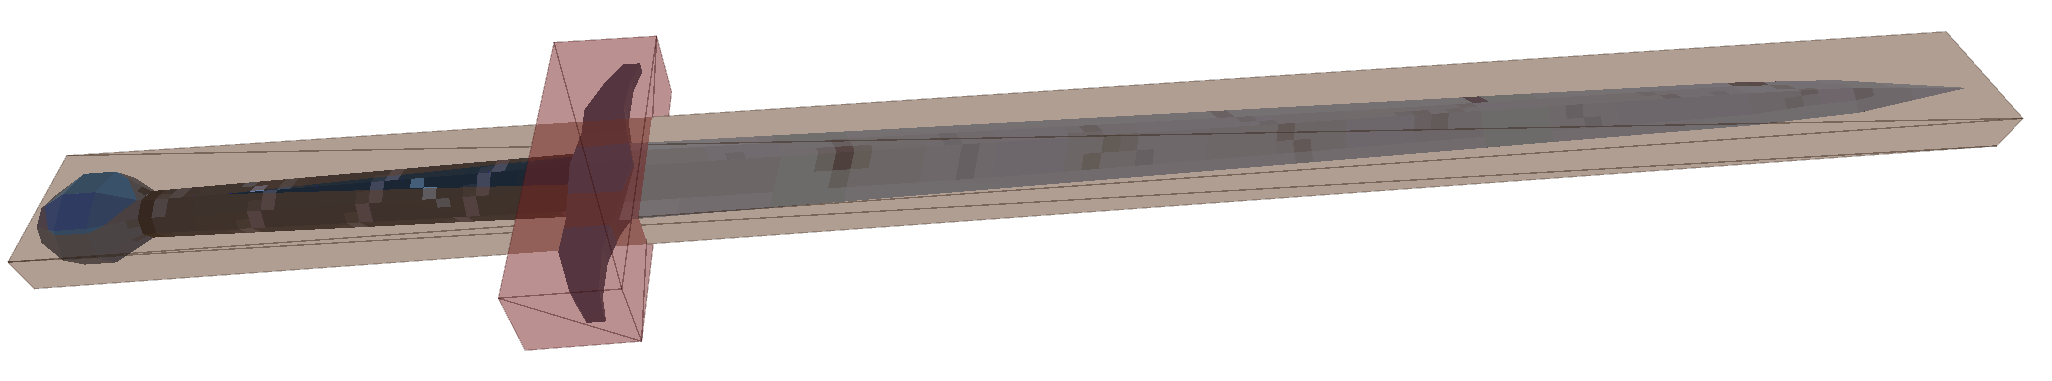
\includegraphics[width=120mm]{../img/swordWithColliders.png}
  \caption{Model meče s rozmístěnými collidery}
  \label{obr05:swordWithColliders}
\end{figure} 
Hoden povšimnutí je značný přesah, jenž jsme colliderům dopřáli - ten je v praxi pro hráče nezaznamenatelný, naopak meč činí méně náchylným na tunelování a obecné nestabilní chování, jež by nastávalo kdyby collidery těsně kopírovaly grafický model.  

Na mnoha místech herní logiky\footnote{Např. v modech pro ovládání meče - viz \ref{interfacesSwordMovementBlockingModuleSubsubsection}.} se meč účastní geometrických výpočtů - v těch s ním typicky pracujeme jako s množinou několika pojmenovaných význačných bodů. Ty vyznačíme zde přímo na modelu meče. Každému z nich bude odpovídat jeden prázdný (pouze s komponentou Transform) podobjekt našeho modelu. Abychom nemuseli úmorně přetahovat jednotlivé Transformy v editoru na každé místo, kde provádíme výpočty, vytvořili jsme komponentu \textit{SwordDescriptor} - ta pro každý význačný bod definuje serializovatelnou proměnnou - stačí tedy každý bod v editoru přetáhnout pouze do této komponenty, cizím objektům dále budeme předávat odkaz na ní.

\bigbreak

Takto definovaný model meče je samostatně existenceschopnou entitou. Nic nám tedy nebrání vytvořit z něj vlastní prefab.

\subsubsection*{Základní struktura} 

Nyní přistupme k hlavnímu objektu meče. Do toho jsme umístili výše popsaný model meče jako dítě. Hlavní objekt je zodpovědný za účast meče ve fyzikální simulaci a za hráčovu schopnost meč ovládat.

Vstup od hráče přijímá, stejně jako šermíř, z komponenty ISwordInput.

Najdeme zde dvě hlavní komponenty fyzikálního systému - nekinematické Rigidbody a ConfigurableJoint.

\textbf{Rigidbody} jsme stanovili váhu 1.5 (typická váha jedenapůlručního meče), později jsme došli k objevu, že pro optimální hráčský zážitek je třeba vypnout gravitaci a ručně nastavit těžiště a \textit{intertiaTensor} - o tom zevrubněji v \ref{swordParameterTweaksSection}.

\textbf{ConfigurableJoint} meči velmi přímočaře poskytl schopnost být držen šermířem - stačí nastavit šermířovo Rigidbody jako \textit{connectedBody} jointu. \textit{Anchor} jsme umístili doprostřed rukojeti - to je bod, ve kterém šermíř meč "drží". 

Z objektového návrhu již známe komponentu \textbf{SwordMovement}, jejímž úkolem je řídit rigidbody a joint tak, aby se meč pohyboval způsobem odpovídajícím hráčskému vstupu.


\subsubsection*{Metoda MoveSword()} \label{swordMovementMoveSwordImplementationSubsection}

Z předchozí kapitoly bychom již měli být seznámeni se strukturou komponenty \textbf{SwordMovement}. Víme tedy, že hostuje množinu modulů - ty slouží jako zdroj high-level instrukcí udávajících cílovou polohu meče. Tyto instrukce jsou SwordMovementu předávány voláním metody MoveSword().

Této metodě je typicky předána nová pozice, od té předchozí libovolně vzdálená, každý snímek (technicky může být volána i několikrát za jeden snímek). Na meč však máme nároky, aby se pohyboval plynule bez náhlých změn rychlosti. Samotná metoda MoveSword() tedy žádný pohyb meče nevykonává - pouze v privátním stavu komponenty komponenty poznačí cílovou pozici, ke které se meč má přibližovat. Vlastní pohyb meče je pak vykonáván pravidelně každý snímek na základě aktuálně platné cílové pozice.

Pozice meče má dvě složky - lineární a rotační. Interně je reprezentujeme zkrátka jako 3D vektor udávající polohu anchoru meče, a kvaternion udávající jeho rotaci kolem anchoru. Pro veřejné rozhraní metody MoveSword() jsme se však rozhodli rotaci reprezentovat formou dvou orientačních bodů - ke kvaternionům se nám zdály jako celkově přívětivější alternativa, která je navíc kompatibilní s maticovými transformacemi.

\begin{figure}[ht]\centering
  \center
  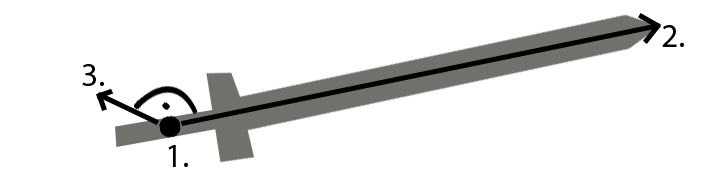
\includegraphics[width=140mm]{../img/diagram-swordPositioning.png}
  \caption{Diagram znázorňující kontrolní body meče}
  \label{obr05:swordPositioningDiagram}
\end{figure} 

Argument MoveSword() má tedy tyto složky:
\begin{enumerate}
    \item \textbf{Poloha rukojeti} (Vektor) - poloha kam se má posunout anchor meče ve světových souřadnicích.
    \item \textbf{Směr meče} (Vektor) - přičtením k Poloze rukojeti dostaneme bod ve světových souřadnicích, kterým má čepel meče procházet.
    \item \textbf{Normála na čepel meče} (Vektor) - pro určení rotace meče kolem jeho osy. Kolmý na Směr meče. Obě hrany ostří čepele se budou nalézat v rovině určené Bodem rukojeti a touto normálou.   
    \item \textbf{Síla držení} (Číslo) - udává jak pevně má meč být držen ve své pozici.
\end{enumerate}

Polohu rukojeti jsme získali přímo, kvaternion pro rotaci vypočteme vestavěnou funkcí:

\begin{lstlisting}[language=C, basicstyle=\fontsize{11}{13}\selectfont\ttfamily]
  UnityEngine.Quaterion.LookRotation(
    forward: SmerMece,
    upwards: NormalaNaCepelMece
  )
\end{lstlisting}

Obě tyto hodnoty a rovněž Sílu držení poznamenáme v privátním stavu, odkud s nimi pracují mechanismy pro vykonávání pohybu.

\subsubsection*{Rotační pohyb}

Nejprve se podívejme odděleně na rotační složku pohybu. Tu bylo možné ponechat téměř zcela v režii ConfigurableJointu.

Na jointu bylo pouze třeba z editoru nakonfigurovat nenulový \textit{angularDrive} a všechny rotační stupně volnosti nastavit jako \textit{Free}. Následně již skript může přepisovat pole \textit{joint.targetRotation} a meč se sám silou jointu bude plynule pohybovat na danou pozici.

Této metodě nečiní problém ani fakt, že je cílová pozice každý snímek novým voláním MoveSword() přepsána - každý snímek joint na meč aplikuje sílu posunující jej k té zrovna aktuální \textit{targetRotation}. 

Jediný větší problém, na který jsme zde narazili, je abnormální souřadnicový systém, který ConfigurableJoint pro targetRotation používá - převod z klasických světových souřadnic, které nám předala MoveSword(), je složitější záležitost a věnujeme mu celou sekci \ref{howToSetJointsTargetRotationSection}. 

Rovněž bylo třeba vyladit parametry jak na rigidbody meče, tak nalézt vhodný \textit{angularDrive}. Následně jsem však získali meč, který je schopen velmi plynulého a celkově pěkného úhlového pohybu a nečiní mu problém ani být realisticky ovlivňován kolizemi s cizími předměty (např. být sražen pod úderem nepřátelského meče) - nad mírou této jeho schopnosti navíc máme vcelku značnou kontrolu skrze konfiguraci \textit{angularDrive} (čím větší \textit{spring}, tím více drží v cílové pozici).

\subsubsection*{Lineární pohyb}

Druhou složkou je lineární pohyb. Podívejme se nyní na ten.

Zde jsme se pokusili, analogicky jako u rotace, pro jednotlivé stupně volnosti nastavit joint jako \textit{Free} a polohu meče kontrolovat pomocí položky \textit{targetPosition}. Narozdíl od rotace, zde se však joint choval nestabilně - pokud jsme cílovou pozici odchýlili příliš daleko od kotvícího bodu, meč začal být v nepředvídatelných intervalech surově vystřelován do dáli. Příčinu takto rozbitého chování se nám nepodařilo odhalit, pro lineární pohyb meče jsme tedy raději zvolili alternativní metodu. 

Pomohla nám proměnná \textit{joint.connectedAnchor}. Ta udává pozici na těle šermíře, ke které je joint svým \textit{anchorem} ukotven. Defaultně je nastavená jako readonly - v editoru jí díky tomu joint může automaticky updatovat, aby souhlasila s nastavenou hodnotou \textit{anchor} a polohou ve světě, kam jsme meč umístili. Zapisovací práva získáme vypnutím\footnote{Vhodné je ho v editoru nechat zapnutý a vypnout jej až programaticky při inicializaci SwordMovement. Takto zachováme pohodlí při práci v editoru.} flagu \textit{joint.autoConfigureConnectedAnchor}. Nakonec je třeba nastavit všechny lineární stupně volnosti na \textit{Locked}.

Zápisem do \textit{joint.connectedAnchor} jsme nyní schopni meč okamžitě přesunout na cílovou pozici. My však potřebujeme pohyb plynule rozložený v průběhu času. 

Vyzkoušeli jsme několik řešení, která jsme následně zavrhli:
\begin{itemize}
  \item knihovnu DOTween - Ta neumožňuje změnit cílovou pozici jakmile tween začal
  \item externí objekt pohybovaný skrze fyzikální systém, na jehož pozici jsme hodnotu connectedAnchoru namapovali - Při dosažení cílové pozice objekt vykazoval jitter, který se nepodařilo odbourat.
\end{itemize}
Řešení, které jsme nakonec použili, bylo jednoduše každý FixedUpdate hodnotu connectedAnchoru posunout o malý zlomek její cesty k cíli - takto: 
\begin{lstlisting}[language=C, basicstyle=\fontsize{11}{13}\selectfont\ttfamily]
  joint.connectedAnchor += AnchorSpeed *
    (targetConnectedAnchor - joint.connectedAnchor) 
\end{lstlisting}
Parametr \textit{AnchorSpeed} je konfigurovaný z editoru. Vzhledem k tomu, že vše probíhá uvnitř FixedUpdate, pohyb je konzistentní.

Jde o velmi triviální řešení, jež neodpovídá realistickému fyzikálnímu chování, avšak pohyb meče se jeví plynule a hráčský zážitek se nezdá výrazněji trpět.

\subsubsection*{Síla držení meče}

Někdy je třeba kromě pozice meče mít kontrolu i nad způsobem, jak je meč držen. Např. v modu blokování potřebujeme, aby byl meč držen pevněji než při sekání, jinak by blokující meč byl tím sekajícím sražen na stranu (sekající se pohybuje a má tedy větší kinetickou sílu). 

Sílu držení meče jsme tedy umožnili definovat spolu s polohou. Jde o volitelný parametr - pokud není dodán, meč se navrací na defaultní sílu držení (která byla z jointu přečtena při inicializaci). Implementace probíhá jednoduše změnou položky \textit{joint.slerpDrive.spring}, používáme k tomu stejnou triviální interpolaci jako pro pohyb \textit{connectedAnchoru} výše.

\subsubsection*{Submoduly}

Již tedy máme představu, jak vnitřně probíhá pohyb meče. Nyní krátce k submodulům, které pro pohyb meče generují instrukce. 

Jak jsme nastínili v \ref{interfacesSwordMovementModulesObjectModelSubsubsection}, moduly jsou zvláštní typ entity, která nedědí z UnityEngine.Object, nýbrž je potomkem SwordMovement.Module. V editoru potřebujeme být schopni nakonfigurovat jeden defaultní modul a libovolně velkou množinu dalších, indexovanou jejich aktivačními klávesami.

Pro spravování indexované množiny objektů jsme implementovali třídu \textit{SerializableDictionary<TKey, TValue>} - ta obsahuje serializovatelný list key-value párů a umožňuje jeho jednoduchý převod na Dictionary. 

Vyvstává však problém - pole v tomto dictionary jsme deklarovali typu SwordMovement.Module - očekáváme, že konkrétní podtřídu vybere uživatel v editoru - Unity však v editoru výběr podtřídy nepodporuje. Naštěstí existuje knihovna SubclassPropertyDrawer \cite{SubclassPropertyDrawer}, která ji je schopna přímočaře doplnit.  

\begin{figure}[ht]\centering
  \center
  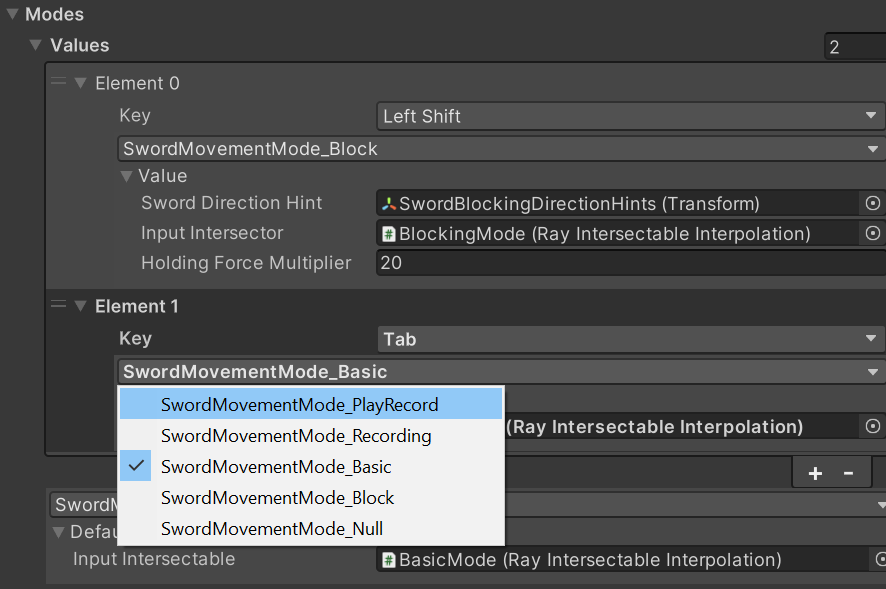
\includegraphics[width=110mm]{../img/swordMovementModulesEditor.png}
  \caption{Editace modulů v unity editoru}
  \label{obr05:swordModulePicker}
\end{figure} 

Správu životního cyklu modulů jsme oddělili do samostatné třídy \textit{ScriptSubmoduleListManager}. Té stačí dodat jejich indexovaný list a následně volat její updatovací callbacky jako by sama byla jediným aktivním modulem. O výběr a updatování aktivního modulu a vše s tím spojené se následně postará sama. 

Chceme-li tedy vytvořit dekorátor, který se vtěsná mezi SwordMovement a jeho moduly, stačí, aby dědil ze SwordMovement.Module a implementoval rozhraní \textit{ISwordMovement}. Původnímu SwordMovement nahradí jeho instanci \textit{ScriptSubmoduleListManager} za novou, ve které se nachází pouze on sám jako defaultní modul, a tu původní instanci ukradne pro sebe - jejím prostřednictvím může nyní originální moduly updatovat sám, aniž by se z jejich pohledu cokoliv změnilo.


\subsubsection*{Shrnutí}

Meč je šermířův nástroj interakce s okolím. Šermíř ho drží v jednom jeho daném bodě - kolem toho může meč rotovat, jeho přesunem se přesunuje meč v prostoru. Toto je umožněno použitím komponenty \textit{ConfigurabeJoint} - především rotační pohyb je díky ní plynulý a fyzikálně realistický. 

Instrukce k pohybu na konkrétní pozici získává meč od modulů své komponenty SwordMovement. Pro ty se nám podařilo umožnit, aby je mohl uživatel konfigurovat z editoru se značnou flexibilitou.

%------------------------------------------------------------------------------------------------------------------------------------------------------------------------------------------------------------------------------------------------------------%
 % xxxxxxxxxxxxxxxxxxxxxxxxxxxxxxxxxxxxxxxxxxxxxxxxxxxxxxxxxxxxxxxxxxxxxxxxxxxxxxxxxxxxxxxxxxxxxxxxxxxxxxxxxxxxxxxxxxxxxxxxxxxxxxxxxxxxxxxxxxxxxxxxxxxxxxxxxxxxxxxxxxxxxxxxxxxxxxxxxxxxxxxxxxxxxxxxxxxxxxxxxxxxxxxxxxxxxxxxxxxxxxxxxxxxxxxxxxxxxxxxxxxxxxxx %
%------------------------------------------------------------------------------------------------------------------------------------------------------------------------------------------------------------------------------------------------------------%


\subsection{Animace šermíře} \label{swordsmanAnimationSubsection}

Šermíře jsme si již navrhli jako kapsli, jež je schopna se působením fyzikálních sil pohybovat herním prostředím a ukotvit k sobě meč. Taková reprezentace je zcela v pořádku z programátorského hlediska, pro hráčův vizuální dojem však není ideální.

Proto jsme tedy v programu Blender \cite{Blender} vytvořili 3D model, který více připomíná humanoidního šermíře. V souladu se standardními postupy jsme mu vytvořili kostru a za její pomoci vytvořili velmi jednoduchou animaci dýchání. Následně jsme model importovali do Unity a umístili mezi potomky šermířského objektu.

Po správném napolohování tohoto detailního těla uvnitř šermířského objektu náš šermíř má adekvátní grafickou reprezentaci, která se pohybuje spolu s ním a je z ní patrné, na kterou stranu je šermíř obrácený. Nyní bychom mohli i přidat animace pro chůzi apod., mezi kterými by mohl přepínat \textit{SwordsmanMovement} v závislosti na aktuálně vykonávaném pohybu - manuální tvorba velkého množství animací však není cílem této práce, omezili jsme se tedy na cyklický běh animace dýchání. 

Detailní tělo dosud figuruje jako čistě kosmetický prvek, který se nijak neúčastní fyzikální simulace. Pokud bychom to takto ponechali, nepovede to k optimálnímu hernímu zážitku - hráč chce pravděpodobně protivníka zasahovat mečem do jeho těla, ne do jakési neviditelné obklopující kapsle. Na jednotlivé kosti\footnote{Rozmístěním colliderů na odpovídající kosti zaručíme, že se při animaci budou pohybovat korektně spolu s šermířovým modelem.} šermířova těla jsme tedy rozmístili komplexní systém colliderů - viz obr. \ref{obr05:swordsmanDetailedColliders}. Kolizní vrstvy jsme nakonfigurovali tak, aby tyto collidery kolidovaly pouze s meči ostatních šermířů, pro interakci s prostředím ponecháváme původní kapsli (té navíc samozřejmě vypneme kolize s meči). 

\begin{figure}[ht]\centering
  \center
  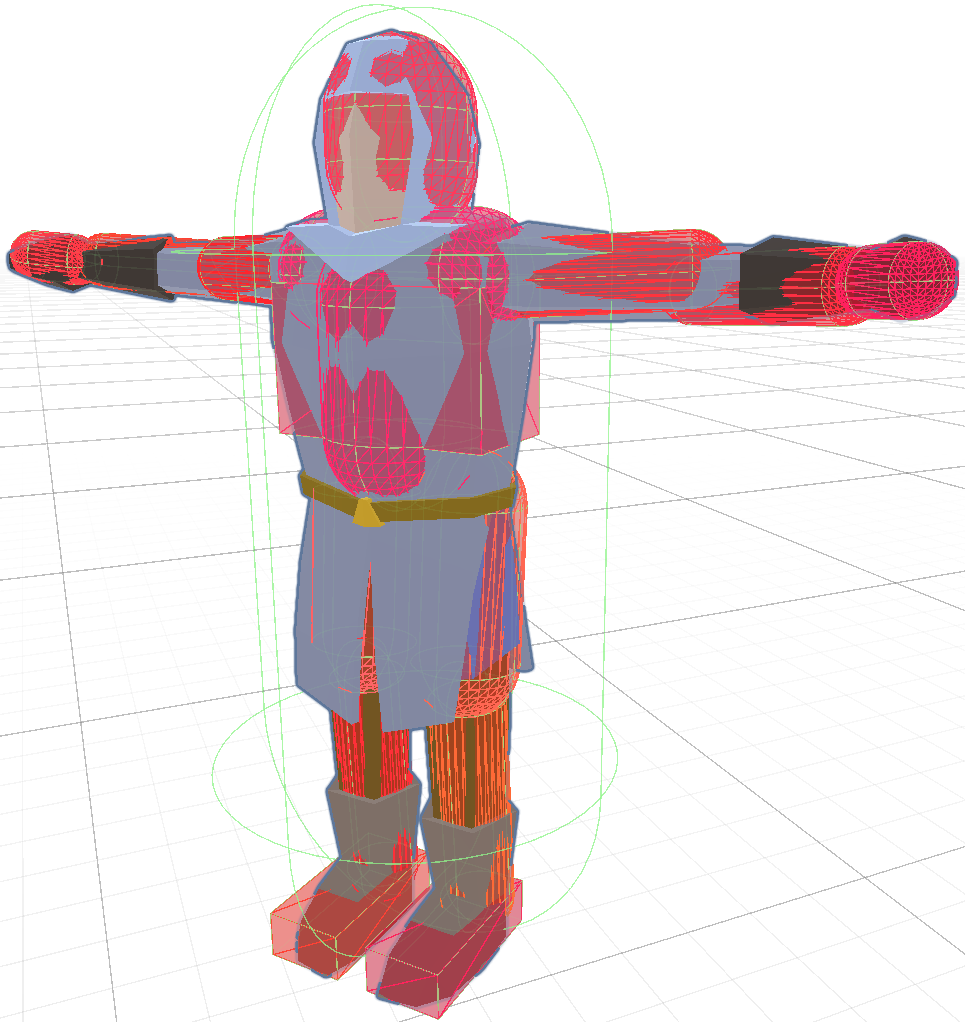
\includegraphics[width=90mm]{../img/swordsmanBodyColliders.png}
  \caption{3D model šermíře s collidery rozmístěnými na kostech}
  \label{obr05:swordsmanDetailedColliders}
\end{figure} 

Jednotlivými animacemi pro pohyb se zaobírat nebudeme, co však je zajímavým tématem, je zaručit, aby šermířovy ruce držely meč - ten se může pohybovat naprosto libovolně, předpřipravené animace tedy není možné použít. 

Zde nám pomůže knihovna Animation Rigging \cite{AnimationRigging}, která byla do Unity představena v nedávných letech. Ta nám poskytuje dodatečnou programovatelnou vrstvu nad vestavěným animačním systémem, skrze kterou můžeme animované objekty ovlivňovat. Najdeme zde mnoho mnoho již předpřipravených komponent, další lze vytvořit jako vlastní skripty.

Těžkou část práce za nás vykonala předpřipravená komponenta \textbf{TwoBoneIKConstraint}. Ta bere na vstupu bod značící cílovou pozici a pro řetězec tří navazujících kostí vypočítá pomocí algoritmu FABRIK \cite{FabrikSolverIK} polohování, které se tváří korektně z hlediska lidské anatomie, zachovává délku kostí a poslední z kostí se při něm nalézá v cílovém bodě. V našem případě oním cílovým bodem je bod, který jsme pro danou ruku vyznačili na rukojeti meče a řetězcem kostí je rameno -> loket -> dlaň.

Pro každou šermířovu ruku jsme tedy vytvořili jednu tuto constraint. Na šermířovo tělo jsme následně umístili komponentu \textit{SwordsmanBodyProceduralAnimation}, jejímž úkolem je tyto constraints updatovat dle bodů získanýmch ze \textit{SwordDescriptoru}. 

Výsledek fungoval velmi dobře - šermířovy ruce skutečně meč na příslušných místech držely. Problém však nastal, pokud se meč ocitl příliš daleko mimo jejich dosah - v takovém případě nastávalo nedefinované chování. K vyřešení tohoto problému jsme tedy napsali dle instrukcí v dokumentaci vlastní constraint \textit{ExtendSwordsmanArmsToReachTheSwordConstraint}, která běží před TwoBoneIKConstraint a jednoduše kosti prodlouží, aby na cílovou pozici vždy dosáhly.


\begin{figure}[ht]\centering
  \center
  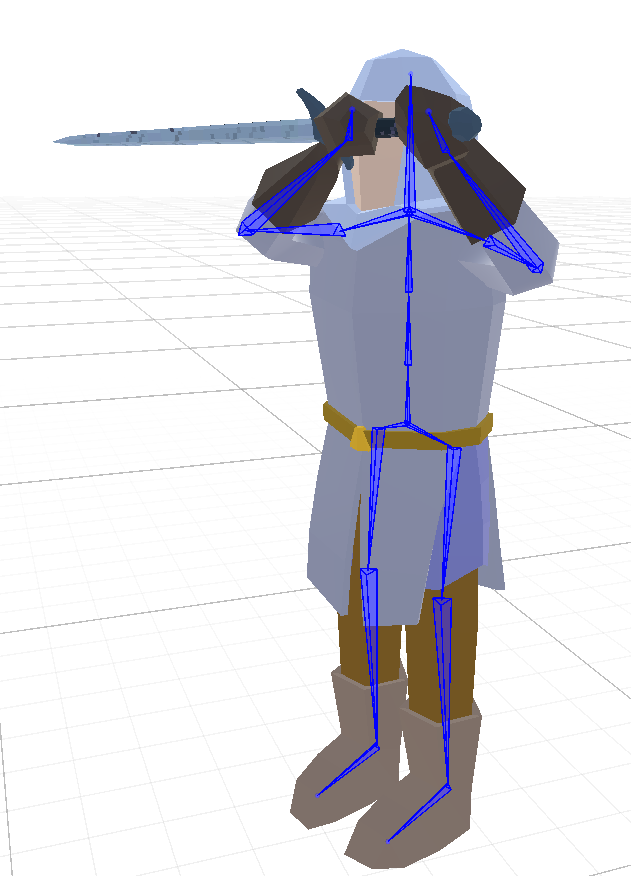
\includegraphics[width=80mm]{../img/swordsmanProceduralAnimation.png}
  \caption{Šermíř držící meč}
  \label{obr05:swordsmanProceduralAnimation}
\end{figure} 


\subsection{Počítání zranění}
\begin{itemize}
  \item Cíl... být tak jednoduché jak jenom jde, ale myslet na rozšiřitelnost do budoucnosti
  \item \textbf{Damageable}
    \begin{itemize}
      \item float HP /*currentHP*/, MaxHP;
      \item poskytuje UnityEventy OnSpawn, OnUpdated, OnDamaged, OnHealed, OnDeath.
      \item metoda ChangeHP(float deltaHP) - řeší damageování i healování
      \item volitelně může celý gameobject automaticky zničit když zemře
    \end{itemize} 
  \item \textbf{AttackDeclaration}
      \begin{itemize}
        \item univerzální deskriptor co popisuje vykonaný útok
        \item zatím velmi jednoduchá, v případě potřeby možné do ní přidat další informace
        \item float Damage, informace (místo+normála) o bodu kde došlo ke zranění
      \end{itemize} 
  \item \textbf{IArmorPiece}
      \begin{itemize}
        \item rozhraní pro jakýkoliv hmotný objekt (obsahující collider), na který může být zaútočeno
        \item z collideru se kanonicky získává jako collider.GetComponentInParent<IArmorPiece>() - může být jeden obecný pro všechny collidery a ten overridovat potomci čistě jenom pro svoje vlastní collidery
        \item nese odkaz na damageable ke kterému patří
        \item metoda ProcessAttack(AttackDeclaration) - vyhodnoť provedený útok!, uber HP na svém Damageable
        \item poskytuje UnityEvent OnAttack
        \item \textbf{BasicArmorPiece} - konkrétní implementace - má DamageMultiplier a MinDamage (dmg pod hranicí je ignorováno), celkově se chová jak by člověk čekal
      \end{itemize} 
  \item \textbf{BasicImpactWeapon}
      \begin{itemize}
        \item jednoduchá zbraň, co útočí na jiný předmět tak, že s ním zkoliduje 
        \item parametry: DamageMultiplier, SecondsBetweenAttacks
        \item při kolizi (OnCollisionEnter) se podívá jestli druhý collider u sebe nemá IArmorPiece - když jo, tak na něm zavolá ProcessAttack()
        \item dmg počítá jako collision.impulse.magnitude*DamageMultiplier, bod zranění je podle collision.GetContact(0)
        \item metoda pro výpočet AttackDeclaration.. virtuální - možné nahradit sofistikovanější implementací
      \end{itemize} 
  
\end{itemize}


%------------------------------------------------------------------------------------------------------------------------------------------------------------------------------------------------------------------------------------------------------------%
 % xxxxxxxxxxxxxxxxxxxxxxxxxxxxxxxxxxxxxxxxxxxxxxxxxxxxxxxxxxxxxxxxxxxxxxxxxxxxxxxxxxxxxxxxxxxxxxxxxxxxxxxxxxxxxxxxxxxxxxxxxxxxxxxxxxxxxxxxxxxxxxxxxxxxxxxxxxxxxxxxxxxxxxxxxxxxxxxxxxxxxxxxxxxxxxxxxxxxxxxxxxxxxxxxxxxxxxxxxxxxxxxxxxxxxxxxxxxxxxxxxxxxxxxx %
%------------------------------------------------------------------------------------------------------------------------------------------------------------------------------------------------------------------------------------------------------------%


\section{Stabilita simulace} \label{simulationStabilitySection}

Nyní by čtenář měl mít hrubý přehled o celkovém vnitřním fungování našeho systému. V této sekci se do detailu zaměříme na nečekané překážky, které nám v průběhu implementace postavil do cesty fyzikální subsystém, a vysvětlíme, jakým způsobem byly překonány.


\subsection{Jak nastavit cílovou rotaci jointu} \label{howToSetJointsTargetRotationSection}
\begin{itemize}
  \item cílová rotace configurable jointu se udává v souřadnicovém systému, co se dost kryptickým způsobem vypočítává podle vícera parametrů, co se na jointu nastavují
  \item když víme kýženou rotaci v globálních souřadnicích, není triviální vypočítat na jejím základě rotaci, co se musí nastavit jako joint.targetRotation
  \item give credits to \href{https://gist.github.com/mstevenson/4958837}{mstevenson}
  \item (insert algorithm here)
  \item (popsat jak přesně algoritmus funguje)
  \item v našem případě jsme potřebovali joint.configuredInWorldSpace=false (= joint konfigurovaný v lokálním prostoru) - jinak se všechno rozbilo když se šermíř otočil 
\end{itemize}

\subsection{Ladění parametrů} \label{swordParameterTweaksSection}
\begin{itemize}
  \item snaha dosáhnout dobrý game feel
    \begin{itemize}
      \item aby meč svižně sekal ze strany na stranu (ne se klátil jako když mácháme s 80kg ledničkou)
      \item aby meč netáhl šermíře pryč z místa kde stojí
      \item aby se všechno nezbláznilo když např. hráč přijde blízko ke stěne a začne dávat vstupy, podle kterých by handle měl být uvnitř té stěny
      \item aby šermíř při blokování držel meč dostatečnou silou, že meč nebude sražen na stranu a opravdu ten úder vyblokuje 
    \end{itemize}

  \item Meč - Parametry, ke kterým jsme se pro optimální hráčský zážitek experimentálně dobrali, jsou tyto: 
    \begin{itemize}
      \item \textit{rigidbody.centerOfMass} - uprostřed rukojeti (totožné s joint.anchor)
      \item \textit{rigidbody.inertiaTensor} - (0.05, 0.05, 0.02)
      \item \textit{joint.rotationDriveMode} - Slerp
      \item \textit{joint.slerpDrive} - spring: 120, damper: 10
    \end{itemize}
    
  \item meči i šermíři jsme nastavili realistickou hmotnost (šermíř 60kg, meč 1.5kg)
  \item \textbf{Svižnost sekání...}
    \begin{itemize}
      \item joint.rotationDriveMode = Slerp - plynulý pohyb, vždy nejkratší cesta mezi dvěma rotacemi
      \item potřeba nenulový joint.angularSlerpDrive.damper (jinak by se meč třásl a nikdy nestabilizoval) ale musí být o dost menší než joint.angularSlerpDrive.spring (když jsou blízko, tak se meč pohybuje strašně líně)
      \item experimentálně binárním vyhledávání jsme našli hodnoty drive=120, damper=10 - ty se chovají pěkně pro normální sekání
      \item další extrémně důležitá věc - vyhrát si s ručním nastavením rigidbody.centerOfMass a rigidbody.inertiaTensor 
        \begin{itemize}
          \item je nezbytně nutné aby se nepřepočítávaly podle toho jak se meči přidávají a odebírají collidery (nezbytně nutné kvůli \ref{swordCollisionsSection} a taky se prostě věci dají jednodušeji ladit když mi v tom automatika nedělá bordel)
          \item pěkně vychází rigidbody.centerOfMass = (0,0,0) a rigidbody.inertiaTensor = nějaké hodně malé číslo - např. (0.05, 0.05, 0.02) (ale všude nenulové protože nula = nekonečno)
        \end{itemize}
    \end{itemize}
  \item \textbf{Aby meč šermíře netahal dopředu apod. ...}
    \begin{itemize}
      \item nastavíme nízkou joint.connectedMassScale - tím pádem se síly, co působí na meč, budou přenášet na šermířovo rigidbody dostatečně redukovaně aby tyhle efekty nebyly pozorovatelné
    \end{itemize}
  \item \textbf{Aby se celkově neděly divné nepřidvídatelnosti...}
      \begin{itemize}
        \item nastavit joint.projectionMode (když by meč měl být na nesplnitelném místě, takhle se místo toho přesune blízko ke hráčovi; fyzikálně nerealistické, ale chová se dost pěkně)
        \item nastavit joint.enablePreprocessing = false (extrémně pomáhá - viz dokumentace (v té prostě říkají, že s ním zapnutým se můžou dít divný věci))
      \end{itemize}
  \item \textbf{Síla blokování...}
    \begin{itemize}
      \item pozorování... při blokování se konzistentně dělo to, že útočící meč blok prolomil (měl stejnej angularDrivem, ale jak byl zrovna uprostřed švihu, tak měl celkově větší energii nebo tak něco)
      \item řešení... při blokování upravit parametry jointu aby blok nešlo prolomit
      \item ukázalo se, že fajn je drive 100krát zvýšit a damper snižit na polovinu (tedy drive=12000, damper=5) (čím větší drive, tím větší síla držení; čím větší damper, tím snadnější blok prolomit; při zvýšení obojího 100krát se to chovalo dost podobně jako v defaultu; jenom snížit damper na setinu původní hodnoty a drive nechat by ale nefungovalo páč pak by se meč strašně třásl atd.)
    \end{itemize}
\end{itemize}

\subsection{Kolize mečů} \label{swordCollisionsSection}
\begin{itemize}
  \item \textbf{nejprve uvést do problematiky}
  \begin{itemize}
    \item fyzikální update běží ve fixně dlouhých krocích
    \item diskrétní detekce kolizí - každý update se jenom koukne jestli collidery vzájemně prochází skrz sebe - když jo, nahlásí kolizi a aplikuje síly aby kolizi vyřešila (podle rychlostí co maj kolidující objekty v daném kroku)
    \item problém - tunelování - tzn. když objekt A letí směrem k objektu B - buď A se pohybuje hodně rychle NEBO B je hodně malý -> stane se, že v 1 snímku ja A na jedné straně objektu B a v druhém už je na druhé straně objektu B - projde skrz, žádná kolize není zdetekována
    \item herní obor kterému tohle nejvíc vadí - \acs{FPS} - potřebují aby letící kulky netunelovaly skrz zdi nebo skrz člověka kterého mají trefit
    \item řešení - spojitá detekce kolizí (continuous collision detection) - podle složitejch fyzikálních vzorečků počítá dráhu objektu v průběhu času mezi snímkama (-> pomalejší než diskrétní, ale kulky s ní netunelujou)
    \item Unity physics spojitou detekci kolizí podporují
  \end{itemize}
  \item \textbf{vysvětlit problém}
  \begin{itemize}
    \item meče... relativně dost malé objekty, pohybují se celkem rychle
    \item -> při diskrétní detekci kolizí často tunelují
    \item řešení: použít spojitou detekci kolizí - \textbf{NEFUNGUJE!}
    \item problém: podle Unity docs... continuous dynamic collision detection bere v úvahu jenom lineární rychlost, \textbf{úhlovou ignoruje} X náš meč se pohybuje především rotačně (je vidět že vážně je koncipovaná především pro letící střely v \acs{FPS} hrách a k ničemu moc dalšímu)
    \item chování spojité detekce v praxi... zdetekuje kolizi celkem dost často v porovnání s tou diskrétní, ale i tak se tunelování děje. taky i když kolizi zdetekuje korektně, většinou nezdetekuje korektně síly - meče často při kolizi tak jako podivně zamrznou 
    \item poslední možná záchrana... \textbf{continuous speculative collision detection} - poslední možnost, kterou Unity nabízí; podle dokumentace by měla brát v úvahu i úhlovou rychlost, jenom tam údajně můžou vznikat ghost kolize
    \item v praxi se ale continuous speculative zdá trpět na tunelování ne o moc líp než diskrétní 
  \end{itemize}
  
  \item \textbf{úvaha - možnosti jak řešit:}
  \begin{itemize}
    \item v každém framu pro všechny meče checkovat jestli třeba náhodou neprošly skrz a když jo, tak zařídit aby se vrátily
      \begin{itemize}
        \item když uděláme chytře, dalo by se naimplementovat efektivněji než jak to zní (checkovat jenom s mečema v okolí - co jsou uvnitř trigger collideru apod.)
        \item jak chceme tu kolizi ručně rozřešit, aby se meče chovaly pěkně realisticky a nerozbila se celková stabilita simulace? - jenom vrátit rigidbody.position na poslední pozici před kolizí se nebude chovat pěkně
      \end{itemize}
    \item drobný skript co poslouchá na kolize a vrací meče na správnou stranu
      \begin{itemize}
        \item pozorování - ve skutečnosti se zpravidla neděje to, že by meče vzájemně protunelovaly úplně bez kolize - kolize je zaznamenána, ale je rozřešena špatně - tak, že meče pošle skrz (to nejspíš i bude důvod proč tuneluje continuous speculative)
        \item myšlenka: když na meči zaznamenáme kolizi, podívat se jakou silou byla rozřešena, a když poslala meče skrz, zvrátit to
        \item problém - callback parametr co dostaneme reportuje o trochu jinou sílu než kterou ve skutečnosti fyzikální systém aplikoval
        \item porovnáním směru kolizní normály a resolvovací síly se dá většinou vydedukovat že procházíme skrz
        \item máme víc informací pro korektní rozřešení kolize než v předchozí možnosti
        \item ALE I TAK - jakou sílu máme zapůsobit aby se pohyb meče zvrátil? - prostě odečíst 2*collision.impact nefunguje - o dost jiná síla než co byla meči dodána kolizí - i kdyby mečům zabránilo projít skrz, budou se pak při kolizích divně klepat apod.
        \item když bychom např. při takové kolizi vraceli transform.position meče na poslední pozici, co měl před kolizí, bude to fyzikálně nerealistické chování, ohrozíme stabilitu simulace apod.
        \item nemusí podchytit všechno tunelování, celkově to není robustní řešení
      \end{itemize}
    \item přidat velký neviditelný collider co meči zabrání projít skrz
      \begin{itemize}
        \item detekci kolize i vypočítání síly pro její rozřešení za nás zvládne udělat fyzikální subsystém
        \item jediné, co musíme udělat, je zařídit, aby ten collider vždycky směřoval správně proti druhému meči
        \item taky potřeba zařídit, aby ten collider nekolidoval s ničím s čím nemá
      \end{itemize}
  \end{itemize}
  \textbf{po troše experimentování a delší úvaze jsme se rozhodli pro možnost s dodatečným neviditelným colliderem}
  \item \textbf{průběh implementace:}
  \begin{itemize}
    \item jak chceme aby to vypadalo: pro každý pár mečů - na jednom z nich velkej collider, co se v reálném čase natáčí tak, aby tomu druhému bráníl v protunelování 
    \item který tvar z primitive colliderů? - vybíráme box collider - jedna jeho hrana bude procházet vlastní osou meče; zbytek collideru je vždycky přesně na opačné straně od osy meče než meč protivníka
    \item pro potřeby zbytku sekce budeme meč považovat za úsečku odpovídající jeho středové ose - spojnici pataČepele<->špička (získaná ze SwordDescriptoru)
    \item dále nechť collider s kterým pracujeme, se nazývá "fixovací collider" či krátce "fixer"
    \item jak definujeme 'na opačné straně'?  
      \begin{itemize}
        \item meče - libovolně mimoběžné úsečky v prostoru
        \item vzít nějakej jeden pevnej bod (např. střed čepele) a ten brát jako reprezentanta, kterému chceme být naproti - nefunguje (spusta případů, kdy to neodpovídá - např. kolize špiček dvou mečů)
        \item co funguje: najít nejkratší spojnici obou mečů - na ní ležej ty 2 body, ve kterých by oba meče potenciálně mohly kolidovat
        \item výpočet:
          \begin{itemize}
            \item meče M, N
            \item X..nejkratší spojnice M,N musí být na oba kolmá - tedy X.direction = M.direction.CrossProduct(N.direction)
            \item nyní stačí řešit soustavu 3 rovnic o 3 neznámých: M.origin + M.t * M.direction + X.direction*X.t = N.origin + N.t * N.direction // kde M.t, X.t, N.t jsou neznámé
            \item tu strčíme do matice a předhodíme gaussovce - knihovna MathNet.Numerics
            \item chceme úsečky -> M.t, N.t sesekáma do intervalu <0,1> - podle nich vypočítáme oba konce výsledné spojnice
          \end{itemize}
      \end{itemize}
    \item pozici kam umístit střed collideru (offset relativní vůči středu meče) získáme takto: 
      \begin{itemize}
        \item let O = nejbližší bod protějšího meče
        \item let P = new Plocha(bod: střed meče, normála:směr meče)
        \item let H = hloubka collideru (parametr od uživatele - vzdálenost od hrany do středu)
        \item return (P.projekce(O).normalized * (-H)) //pro globální pozici přičíst střed meče
      \end{itemize}
    \item rotaci získáme jako Quaternion.AngleAxis(45f, bladeDirection) * Quaternion.LookRotation(offsetCollideruOdStředuMeče, bladeDirection)
    \item takhle tu pozici collideru updatujeme každej FixedUpdate
    \item \textbf{problém} - když meče během 1 snímku protunelujou, collider okamžitě přeskočí na druhou stranu a ničemu nepomůže
    \item řešení: pamatujeme si jeho poslední offset proti středu meče - pokud se mezi 2 snímkama ostře změní (offset.Dot(lastOffset) < 0), tak nově spočítanej offset znegujeme
    \item existujou okrajové případy, co to rozbijou (např. úplně první volání FixedUpdate) - řešení: tuhle negaci provádíme jenom pokud je nejkratší spojnice obou mečů dostatečně krátká (limit konfigurovaný uživatelem, 0.4 metru funguje rozumně)
    \item \textbf{Další problém} - občas se stane, že meč protuneluje na druhou stranu meče a jakoby se skřípne mezi mečem a jeho fixerem - řešení: přidat collideru přesah - velikost navíc se kterou ale jeho pozicovač nekalkuluje (-> místo jenom do středu meče sahá fixer trochu dál)
    \item \textbf{Jak zařídíme, aby collisionFixer kolidoval jenom se správným mečem a s ničím jiným?}
      \begin{itemize}
        \item první řešení, co člověka napadne - dát je na Layer, co nemá nastavené kolize vůbec s ničím, a selektivně zavolat Physics.IgnoreCollision(fixer, targetSword, false) - to ale vůbec nic nedělá, kolize pořád nevznikají
        \item \textbf{řešení:} separátní Layery: CollisionFix, Sword - Sword koliduje s hodně věcma, CollisionFix jenom se Sword -> musíme přidat velký trigger collider - ten včas disabluje kolize se všema mečema co nejsou ten cílový, které se nachomýtnou poblíž
      \end{itemize}
    \item \textbf{fixovací collider umístíme přímo do meče jako jeho podobjekt}
      \begin{itemize}
        \item -> všechny kolize s fixerem povedou k působení síly přímo na rigidbody meče (a síla bude přesně ta co je realistická)
        \item \textbf{problém:} dodatečnej collider, co se ještě pořád chaoticky otáčí, totálně rozhodí balance meče - řešení: \textbf{potřeba mít nastavený custom centerOfMass a inertiaTensor aby se nepřepočítávaly podle fixeru!} 
      \end{itemize}
    \item \textbf{Jak se tedy výsedek používá z pohledu uživatele?}
      \begin{itemize}
        \item Na meč stačí přidat komponentu CollisionFix - ta automaticky zařídí, aby se vytvořil fixer pro každej další meč, co se nachomítne poblíž (fixer je umístěnej do jednoho z těch dvou mečů - náhodně vybráno který)
        \item v případě že je meč zničený, všechny fixery co na něj cílily, se automaticky zničej taky
        \item CollisionFix by měl v defaultu být nakonfigurovanej funkčně, ale uživatel na něm může ladit parametry pro fixer (hloubku, přesah apod.), radius ve kterém se fixery vytvářejí ; taky může přidat list objektů co se z fixu mají vynechat
      \end{itemize}
  \end{itemize}
\end{itemize}

%------------------------------------------------------------------------------------------------------------------------------------------------------------------------------------------------------------------------------------------------------------%
 % xxxxxxxxxxxxxxxxxxxxxxxxxxxxxxxxxxxxxxxxxxxxxxxxxxxxxxxxxxxxxxxxxxxxxxxxxxxxxxxxxxxxxxxxxxxxxxxxxxxxxxxxxxxxxxxxxxxxxxxxxxxxxxxxxxxxxxxxxxxxxxxxxxxxxxxxxxxxxxxxxxxxxxxxxxxxxxxxxxxxxxxxxxxxxxxxxxxxxxxxxxxxxxxxxxxxxxxxxxxxxxxxxxxxxxxxxxxxxxxxxxxxxxxx %
%------------------------------------------------------------------------------------------------------------------------------------------------------------------------------------------------------------------------------------------------------------%



\section{Demo hra}
\begin{itemize}
  \item Pro testování a demonstraci funkčnosti našeho konceptu jsme vytvořili ukázkovou hru
  \item herní svět - aréna + okolní les
  \item PC - šermíř, může chodit po světě a používat libovolně meč
  \item v aréně lze bojovat s jednoduchými NPC nepřáteli
  \item všechny modely a textury byly vytvořené autorem této práce a vztahuje se na ně MIT licence jako na všechno ostatní
\end{itemize}

\subsection{Herní svět}
\begin{itemize}
  \item les jsou jenom pěkné kulisy
  \item V aréně jsou sloupy s čudlíkama - po jejich stisknutí mečem se uvnitř arény spawne nepřítel
  \item několik druhů nepřátel: trénovací panák, mečotoč, rytíř (podrobně rozebereme v jejich vlastních sekcích)
\end{itemize}

\subsection{GUI}
\begin{itemize}
  \item všechno pomocí klasického gameobjectového UI
  \item PauseMenu.. naprostá klasika - root čeká na zmáčknutí Esc - pak nastaví Time.timeScale = 0 a enabluje svoje potomky
  \item DieScreen.. taky nic zajímavého - při spuštění tweenem přes obrazovku zobrazí hardcoded bloodstains sprite a "Press F to Restart" (reloadne scénu)
  \item HUD.. healthbar + bloodstains.. dvě drobné komponenty, nad nima kontroler - poskytuje callback, co se musí přidat do OnUpdate na nějakém Damageable
\end{itemize}


\subsection{Statičtí nepřátelé}
\begin{itemize}
  \item Nemohou se hýbat, stojí tam, kde byli spawnutí
  \item \textbf{Trénovací panák}
    \begin{itemize}
      \item Jenom stojí a bere damage dokud není zničený
    \end{itemize}
  \item \textbf{Mečotoč}
    \begin{itemize}
      \item Koule, co rotuje dokola na tyči (uchycené configurable jointem, který má nastavenou targetVelocity a angularDrive)
      \item Ke kouli je jointama připojených 1 nebo víc mečů - ty způsobují dmg úplně stejně jako šermířův meč
      \item Na jointu meče - vysoká connectedMassScale -> hráč může zachytit meč mečotoče o ten svůj a celý pohyb mečotoče tím zastavit, příp. tlačit proti směru rotace
      \item Při spawnu randomizován počet mečů, odkud kam se koule posunuje po tyči, a jakou má volnost rotace (- SwordmillRandomizer)
    \end{itemize}
  \item \textbf{IRandomizable}
  \begin{itemize}
    \item Libovolný skript, myšlenka je, že by měl při spawnu randomizovat parametry svého gameobjectu
    \item Spawnovací skript na entitě ihned po spawnu (tedy před zavoláním Start()) iteruje přes všechny IRandomizable ve všech potomcích a volá na nich metodu Randomize()
    \item Implementován např. pro randomizaci transformu (rotace, velikost trénovacího panáka, apod.), randomizaci HP, randomizaci mečotoče
    \item Ten samý systém je použitý i pro náhodou generaci palisády, co ohraničuje arénu
  \end{itemize}
\end{itemize}


\subsection{Rytíř} \label{knightEnemySubsection}
\begin{itemize}
  \item vychází z prefabu pro hráče - jenom nahrazuje ovládání klávesnicí a myší za počítačový algoritmus
  \item taky nemá žádnou vazbu na hráčovo GUIčko (healthbar, bloodstains, death screen apod.) a není k němu spárovaná žádná kamera
  \item v rootu komponenta SwordsmanAI - ovladač
  \item \textbf{pohyb po terénu}
    \begin{itemize}
      \item používá standardní Uniťácký NavMesh - aby mohlo najednou být spawnutých víc rytířů najednou - co se vyhýbají jeden druhému a okolním překážkám
      \item uvnitř arény jsme umístili NavMeshSurface, hráčovi a statickým nepřátelům jsme přidělili NavMeshObstacle -> rytíři jsou schopní se navigovat po aréně a vyhýbat se veškerým překážkám
      \item NavMeshAgent... agent.updatePosition = agent.updateRotation = agent.updateUpAxis = false
      \item Agent nijak nemodifikuje transform rytíře - místo toho řidicí skript kouká na jeho vyžádanou pozici a podle ní určuje hodnotu co nastaví do InputSimulatoru, ze kterého rytířův SwordsmanMovement bere vstup ; obdobně jako v \href{https://docs.unity3d.com/Manual/nav-CouplingAnimationAndNavigation.html}{tomhle manuálu} 
      \item má nastavený nějaký transform jako cíl - Agentovi nastavuje aby se k němu snažil přiblížit
      \item když je k cíli dostatečně blízko, tak agenta ignoruje a místo toho jenom stojí a dává pozor aby byl otočenej směrem na cíl
    \end{itemize}
  \item \textbf{ovládání meče}
      \begin{itemize}
        \item \textbf{pořídili jsme několik nahrávek pohybů meče}
          \begin{itemize}
            \item komponenta co se vecpe mezi SwordMovement a jeho submoduly - odchytává veškerá volání MoveSword() a reportuje jejich parametry do UnityEventu
            \item parametry čte druhá komponenta - každý jednotlivý struct s argumentama převede do souřadnic relativních vůči transformu šermíře, přidá timestamp, a celou nahrávku ukládá jako pole do JSON texťáku (přes Newtonsoft.Json)
          \end{itemize}
        \item \textbf{přehrávání nahrávek}
          \begin{itemize}
            \item ve SwordsmanAI se v editoru nastaví pole nahrávek, co se mají přehrávat jako TextAssety
            \item SwordsmanAI nejdřív deserializuje všechny nahrávky
            \item potom násilně ve SwordMovementu vyhází původní Submoduly a vymění je za jediný defaultní SwordMovementMode\_PlayRecord
            \item tomuhle submodulu předá seznam nahrávek co má přehrávat - submodul si pokaždé jednu náhodně vybere a tu přehrává
            \item přehrávání nahrávek - submodul se řídí podle timestampů, hodnoty co jsou v záznamu převádí zpátky do globálních souřadnic podle transformu rytíře
          \end{itemize}
      \end{itemize}
    \item máme tedy \acs{NPC} rytíře, co je schopný samostatně chodit po terénu a nebezpečně mávat mečem, drtivou většinu vnitřní logiky sdílí s \acs{PC}
\end{itemize}


\section{Shrnutí}

Dokončili jsme implementaci naší práce. Meč i šermíř jsou plnohodnotnými prvky fyzikální simulace se všemi výhodami, které toto přináší např. pro možnosti interakce s okolním prostředím. Pro meč jsme implementovali dva základní submoduly ovládání - sekání a blokování. Pro tělo šermíře jsme vytvořili za použití standardního balíčku Animation Rigging procedurální animaci, která zajišťuje, aby kosmeticky "držel" meč. Rovněž jsme načrtli systém životů a výpočtu zranění.

Velkou výzvou bylo zajistit realistické \textbf{chování mečů při kolizích}. Žádná z metod detekce kolizí, které Unity nabízí, nebyla schopna zcela zabránit tunelování. Řešením bylo pro každý pár mečů vytvořit dodatečný "velký" collider, který se nacházel na jednom z mečů a natáčel se dle polohy toho druhého. Dalším netriviálním úkolem bylo vyladit fyzikální parametry, aby bylo dosaženo plynulého pocitu při švihu mečem. 

Pro praktickou demonstraci možností našeho systému jsme následně vytvořili ukázkovou hru. Hráč zde může v prostředí fantasy arény zápasit s jednoduchými počítačem řízenými protivníky, kteří používají standardní NavMesh pro orientaci v terénu a útočí přehráváním přednahraných pohybů meče. 
